\chapter{免疫制剂}

\begin{framed}
\noindent\textbf{【知识体系】}
\begin{center}
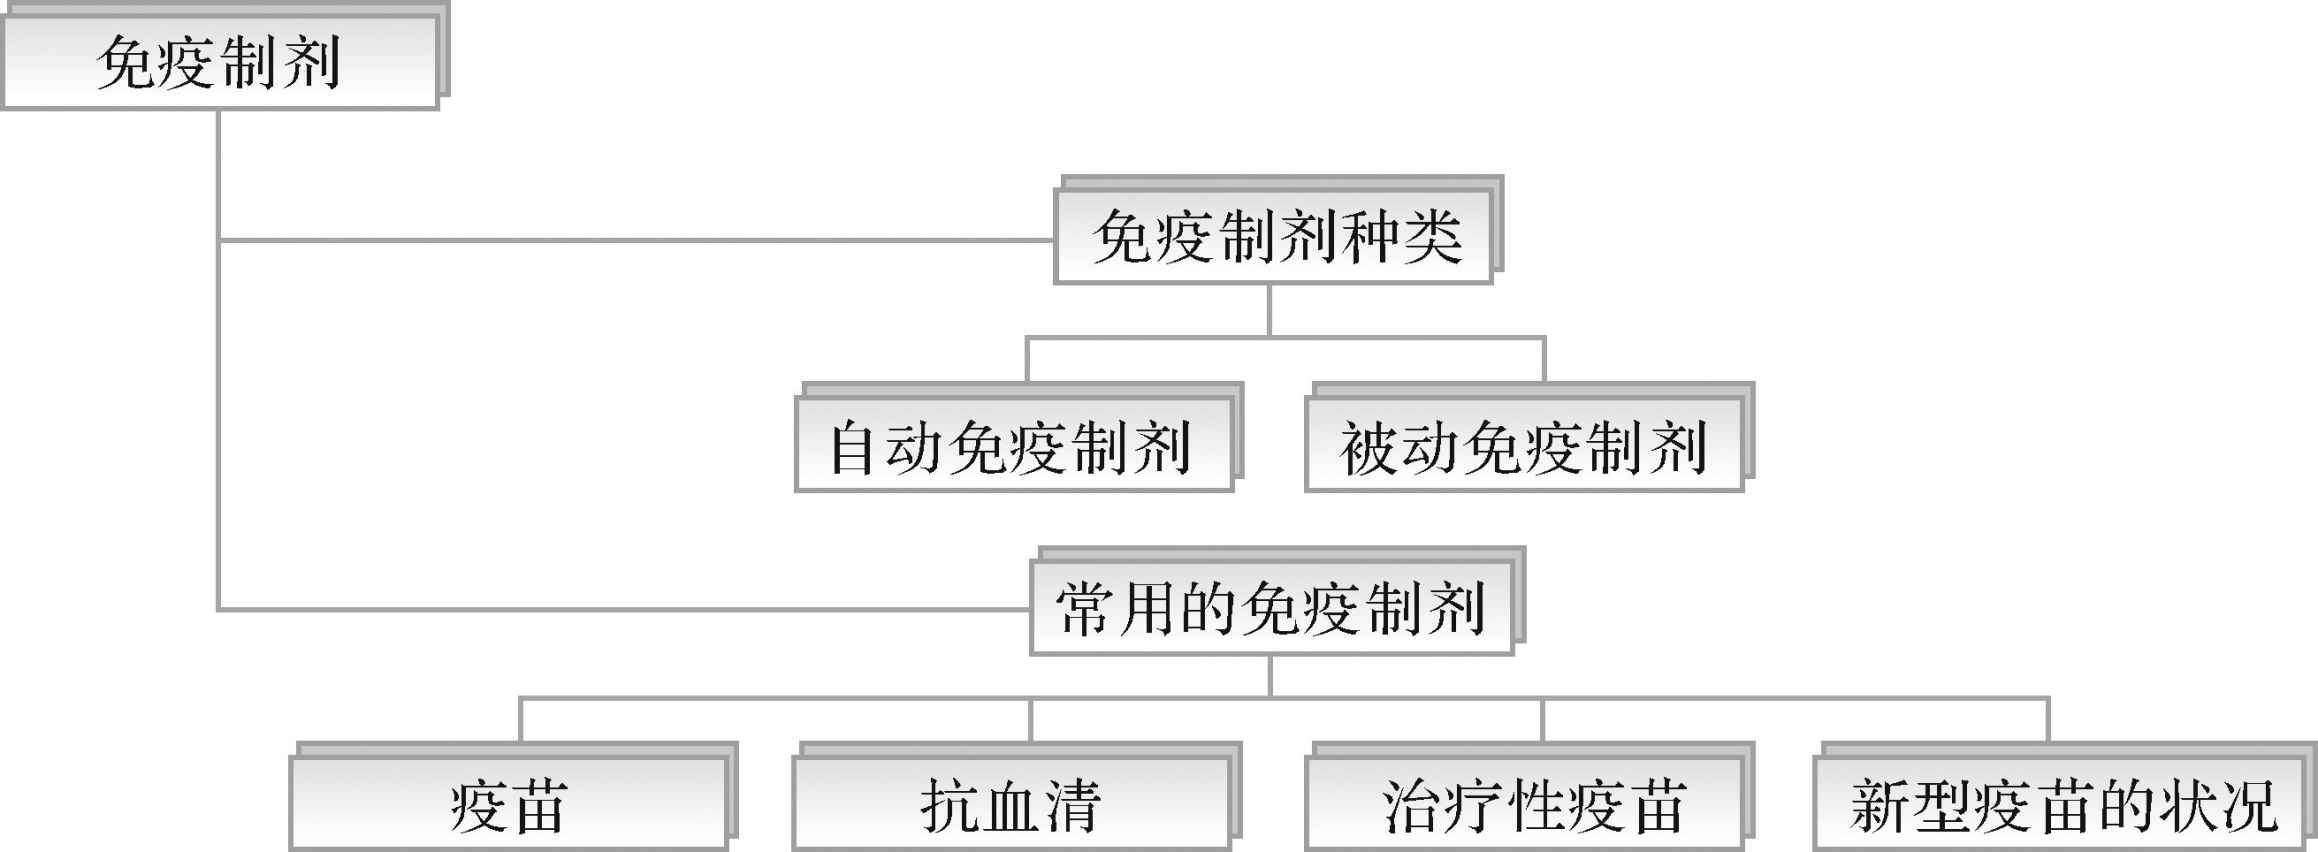
\includegraphics{./images/Image00185.jpg}
\end{center}
\noindent\textbf{【课前思考】}

1.你知道常用的疫苗有哪些吗?你自己使用过哪些?为何需要众多的疫苗?

2.你知道治疗性疫苗吗?其作用机理如何?

3.被狗咬伤后要注射什么?有什么注意点吗?

\noindent\textbf{【本章重点】}

1.常用疫苗的使用特点;

2.抗血清使用的注意点。

\noindent\textbf{【教学目标】}

1.熟悉疫苗、抗血清种类及使用特点;

2.治疗性疫苗的特点及种类。
\end{framed}

\section{免疫制剂的种类}

免疫制剂是应用普通的或以基因工程、细胞工程、蛋白质工程、发酵工程等生物技术获得的微生物、细胞及各种动物和人源的组织和液体等生物材料制备,用于人类疾病预防和治疗的生物制剂,接种后可使机体获得免疫力。免疫制剂可分为:自动免疫制剂和被动免疫制剂。


\subsection{自动免疫制剂}

自动免疫制剂主要是指疫苗,是将病原微生物(如细菌、立克次氏体、病毒等)及其代谢产物,经过人工减毒、灭活或利用基因工程等方法制成的,用于预防传染病。

疫苗包括:灭活疫苗(死疫苗)、减毒素疫苗、类毒素、亚单位疫苗、基因工程疫苗、合成肽苗、DNA苗、转基因植物苗等。


\subsection{被动免疫制剂}

给机体输入含有特异性抗体的免疫血清或细胞因子,把现成的免疫力转移给机体,以预防相应疾病的发生,称为人工被动免疫,这类生物制品称为“被动免疫制剂”。常用的人工被动免疫制剂有:抗毒素、抗血清、人免疫球蛋白制剂及细胞因子等。

\section{常用的免疫制剂}


\subsection{疫苗}

\textbf{(一)伤寒疫苗}

【接种对象】
主要用于部队、港口、铁路沿线工作人员,下水道、粪便、垃圾处理人员,饮食行业、医务防疫人员及水上居民或有本病流行地区的人群。

【不良反应】 局部可出现红肿,有时有寒战、发热或头痛。一般可自行缓解。

【禁忌证】过敏和免疫抑制。

【制剂与免疫程序】

1.伤寒疫苗(Typhoid Vaccine)

本品系用伤寒沙门菌培养后,取菌苔制成悬液,经甲醛杀菌,以PBS稀释制成。为乳白色混悬液,含苯酚防腐剂。

免疫程序:于上臂外侧三角肌附着处皮下注射。初次注射本疫苗后,需注射3针,每针间隔7~10天。注射剂量如下:1~6周岁:第1针0.2mL,第2针0.3mL,第3针0.3mL;7~14周岁:第1针0.3mL,第2针0.5mL,第3针0.5mL;14周岁以上:第1针0.5mL,第2针1.0mL,第3针1.0mL。加强注射剂量与第3针相同。

2.伤寒副伤寒甲联合疫苗(Typhoid and Paratyphoid A Combined Vaccine)

本品系用伤寒沙门菌、副伤寒甲型沙门菌分别培养,取菌苔制成悬液,经甲醛杀菌,以PBS稀释制成。为乳白色混悬液,含苯酚防腐剂。免疫程序同伤寒疫苗。

3.伤寒副伤寒甲乙联合疫苗(Typhoid and Paratyphoid A&B Combined
Vaccine)

本品系用伤寒沙门菌、副伤寒甲型沙门菌、副伤寒乙型沙门菌分别培养,取菌苔制成悬液,经甲醛杀菌,以PBS稀释制成。为乳白色混悬液,含苯酚防腐剂。免疫程序同伤寒疫苗。

4.伤寒Vi多糖疫苗(Vi Polysaccharide Typhoid Vaccine)

本品系用伤寒沙门菌培养液纯化得Vi多糖,经用PBS稀释制成,为无色澄明液体。

免疫程序:上臂外侧三角肌肌内注射;注射1针,剂量为0.5mL。

\textbf{(二)脑膜炎球菌疫苗}

【接种对象】 参见具体疫苗。

【不良反应】 本疫苗反应轻微,偶有短暂低热,局部稍有压痛感,可自行缓解。

【禁忌证】(1)有癫痫、惊厥及过敏者;(2)患脑部疾患、肾脏病、心脏病及活动性结核者;(3)患急性传染病及发热者。

【制剂与免疫程序】

1.A群脑膜炎球菌多糖疫苗(Group A Meningococcal Polysaccharide)

本品系用A群脑膜炎奈瑟菌培养液,经提取获得的荚膜多糖抗原,纯化后加入适宜稳定剂冻干制成,为白色疏松体,复溶后为澄明液体。接种对象为6个月~15周岁少年儿童。免疫程序见免疫接种总论。

2.A群C群脑膜炎球菌多糖疫苗(Group A+C Meningococcal Polysaccharide
vaccine)

本品系用A群及C群脑膜炎奈瑟菌培养液,经提纯获得A群及C群多糖抗原并加入适宜稳定剂后冻干制成的多糖疫苗。成品外观为白色疏松体,加入所附PBS后可迅速溶解,溶液澄明无异物。接种对象为2周岁以上儿童及成人,在流行区的2岁以下儿童可进行应急接种。

\textbf{(三)钩端螺旋体疫苗}

【接种对象】 流行地区7~60岁的人群。

【不良反应】
全身及局部反应一般轻微,偶有发热及局部疼痛、红肿,一般可自行缓解。

【禁忌证】(1)发热,患急性传染病、严重心脏病、高血压、肝脏疾病、肾脏疾病、神经系统和精神疾病者;(2)妊娠期、哺乳期妇女;(3)有过敏史者;(4)月经期暂缓注射。

【制剂与免疫程序】

钩端螺旋体疫苗(Leptospira Vaccine)

本疫苗系用各地区主要的钩端螺旋体流行菌型的菌株,经培养杀菌后制成单价或多价。为微带乳光的液体,含苯酚防腐剂。

免疫程序:上臂外侧三角肌附着处皮下注射。共注射2针,间隔7~10天。第1针注射0.5mL,第2针注射1.0mL。7~13周岁用量减半。必要时7周岁以下儿童可酌量注射,但不超过成人量的1/4。

\textbf{(四)鼠疫疫苗}

【接种对象】 疫区或通过疫区的人员。

【不良反应】
接种后反应轻微,少数人划痕处会出现浸润,一般不影响活动,个别人体温可能稍有升高,一般可自行消退。

【禁忌证】
(1)患严重疾病、免疫缺陷症及用免疫抑制剂治疗者;2)妊娠期或6个月内的哺乳期妇女。

【制剂与免疫程序】

皮上划痕用鼠疫活疫苗(lague Vaccine(Live) for Percutaneous
Scarification)本品系用鼠疫菌弱毒菌株经培养后收集菌体,加入稳定剂冻干制成。为白色或淡黄色疏松体,复溶后为均匀悬液。本品仅供皮上划痕用,严禁注射!开启疫苗瓶和接种时,切勿使消毒剂接触疫苗。

免疫程序:按标示量加入氯化钠注射液溶解。每瓶20次人用剂量者加入1.0mL,10次人用剂量者加入0.5mL,复溶后的疫苗在3小时内用完。在上臂外侧三角肌上部附着处皮上划痕接种。在接种部位上滴加疫苗,每1次人用剂量0.05mL。用消毒针划成“井”字,划痕长度约1~1.5cm,应以划破表皮稍见血迹为宜。划痕处用针涂压10余次,使菌液充分进入划痕内。接种后局部应裸露至少5分钟。14周岁以下儿童,疫苗滴于两处划两个“井”字。“井”字间隔2~3cm。接种人员每年应免疫1次。

\textbf{(五)炭疽疫苗}

【接种对象】
炭疽常发地区人群,皮毛加工与制革个人、放牧员以及其他与牲畜密切接触者。

【不良反应】
接种后局部可出现微红,不需处理;极个别者可出现低热,但能自行消退。如出现持续性体温升高,而局部出现脓肿者,应做对症处理。

【禁忌证】(1)患严重疾病、严重皮肤病者;(2)有免疫缺陷症及接受免疫抑制剂治疗者;(3)有过敏反应史者。

【注意事项】(1)本品仅供皮上划痕用,严禁注射;(2)开启疫苗瓶和接种时,切勿使消毒剂接触疫苗;(3)疫苗有摇不散的菌块或疫苗瓶有裂纹者,均不得使用;(4)用前应将疫苗充分摇匀,消毒皮肤只可用乙醇,不可用碘酒;(5)疫苗瓶开启后,应于3小时内用完,剩余的疫苗应废弃;(6)剩余疫苗、空疫苗瓶及用具,需用3%碱水煮沸消毒30分钟;(7)严禁冻结。

【制剂与免疫程序】

皮上划痕人用炭疽活疫苗(Anthrax Vaccine(live) for Percutaneous
Scarification)

本品系用炭疽芽孢杆菌的弱毒株经培养、收集菌体后稀释制成。为灰白色均匀悬液。

免疫程序:(1)在上臂外侧三角肌附着处皮上划痕接种。用消毒注射器吸取疫苗,在接种部位滴2滴,间隔3~4cm,划痕时用手将皮肤绷紧,用消毒划痕针在每滴疫苗处做“井”字划痕,每条痕长约1~1.5cm。划破表皮以出现间断小血点为度。(2)用同一划痕针反复涂压,使疫苗充分进入划痕处,接种后局部至少应裸露5~10分钟,然后用消毒干棉球擦净。(3)接种后24小时划痕部位无任何反应者应重新接种。

\textbf{(六)布氏菌疫苗}

【接种对象】
与布氏菌病传染源有密切接触者,每年应免疫一次。布氏菌素反应阳性者可不予接种。

【不良反应】
接种后局部反应轻微,少数人划痕处会出现轻度浸润,一般不影响活动。个别人体温稍有增高,一般可自行消退。如因使用途径错误,出现类似急性布氏菌病症状者,要按急性布氏菌病进行彻底治疗。

【禁忌证】

(1)患严重疾病、免疫缺陷症及接受免疫抑制治疗者。

(2)妊娠期及6个月内的哺乳期妇女。

【注意事项】

(1)本品仅供皮上划痕用,严禁注射!

(2)开启疫苗瓶和接种时,切勿使消毒剂接触疫苗。

(3)疫苗瓶有裂纹或标签不清者,均不得使用。

【制剂与免疫程序】

皮上划痕人用布氏菌活疫苗(Brucellosis Vaccine(Live) for Percutaneous
Scarification)

本品系用布氏菌的弱毒菌株经培养、收集菌体加入稳定剂后冻干制成。为乳白色疏松体,复溶后为均匀悬液。

免疫程序:(1)每瓶加入0.5mL氯化钠注射液,复溶后的疫苗应在3小时内用完,剩余的疫苗应作废。(2)上臂外侧三角肌上部附着处皮上划痕接种。在接种部位滴加疫苗,每1次人用剂量0.05mL,应以划破表皮微见血迹为宜。划痕处用针涂压10余次,使菌苗充分进入划痕内。接种后局部应裸露至少5分钟。(3)10岁以下儿童及复种者疫苗滴于一处划一个“井”字,10岁以上初种者疫苗滴于两处划两个“井”字,间隔2~3cm。

\textbf{(七)卡介苗}

【接种对象】 出生3个月以内的婴儿或用5IU
PPD试验阴性的儿童(PPD试验后48~72小时局部硬结在5mm以下者为阴性)。

【不良反应】
接种后两周左右,局部可出现红肿浸润,若随后化脓,形成小溃疡,可用1%龙胆紫涂抹,以防感染。一般8~12周后结痂,如遇局部淋巴结肿大软化形成脓疱,应及时诊治。

【禁忌证】

(1)患结核病、急性传染病、肾炎、心脏病者。

(2)患湿疹或其他皮肤病者。

(3)患免疫缺陷症者。

【注意事项】

(1)严禁皮下或肌内注射!

(2)疫苗瓶有裂纹者不得使用。

(3)接种对象必须详细登记姓名、性别、年龄、住址、疫苗批号及亚批号、制造单位和接种日期。

(4)接种BCG的注射器针头要专用,不得用作其他注射,以防止发生化脓反应。

(5)使用时BCG应注意避光。

【制剂与免疫程序】

皮内注射用卡介苗(BCG Vaccine for Intradermal Injection)

本品系用卡介菌经培养后收集菌体,加入稳定剂冻干制成。为白色疏松体或粉末,复溶后为均匀悬液。免疫程序参考接种总论。

\textbf{(八)白喉疫苗}

【接种对象】 参考具体疫苗。

【不良反应】注射本品后局部可有红肿、疼痛、发痒或有低热、疲倦、头痛等,一般不需要特殊处理即可消退,如有严重反应及时诊治。

【禁忌证】

(1)有癫痫、神经系统疾病及惊厥者。

(2)急性传染病(包括恢复期)及发热者,暂缓注射。

(3)有过敏史者。

【注意事项】

(1)使用时应充分摇匀,如出现摇不散的凝块、异物、疫苗曾经冻结、疫苗瓶有裂纹或标签不清者,均不得使用。

(2)注射后局部可能有硬结,1~2个月即可吸收,注射第2针时应换另侧部位。

(3)应备有肾上腺素等药物,偶有发生严重过敏反应时急救用。接受注射者在注射后应在现场休息片刻。

(4)严禁冻结。

【制剂与免疫程序】

1.吸附白喉疫苗(Diphtheria Vaccine,Adsorbed)

白喉疫苗是用白喉杆菌菌种,在适宜的培养基中产生的毒素经甲醛脱毒、精制,加入氢氧化铝佐剂制成。为白色均匀悬液,长时间放置后佐剂下沉,溶液上层无色澄明,但经振摇后能均匀分散,含防腐剂。接种对象为6个月~12岁儿童。

注射部位:上臂三角肌肌内注射。

免疫程序与剂量如表\ref{tab12-1}所示。 

\begin{table}[htbp]
    \centering
    \caption{吸附白喉疫苗的免疫程序}
    \label{tab12-1}
    \begin{tabular}{llll}
        \toprule
免疫程序&年份&针次&剂量/mL\\
\midrule
\multirow{2}*{全程免疫}&第1年&第1针(间隔4~8周)第2针&0.5,0.5\\
~&第2年&注射1针&0.5\\
加强免疫&3~5年后&加强1针&0.5\\
\bottomrule
    \end{tabular}
\end{table}

2.吸附白喉疫苗(成人及青少年用)(Diphtheria Vaccine for Adults and
Adolescents,Adsorbed)

本品系由白喉类毒素原液加入氢氧化铝佐剂制成。为乳白色均匀混悬液,长时间放置佐剂下沉,溶液上层应无色澄明,但经振摇后能均匀分散,含防腐剂。接种对象为12岁以上的人群。

免疫程序:注射1次,注射剂量0.5mL。

3.吸附白喉破伤风联合疫苗(Diphtheria Tetanus Combined
Vaccine,Adsorbed)

本品系用白喉类毒素原液和破伤风类毒素原液加入氢氧化铝佐剂制成。为乳白色均匀悬液,长时间放置佐剂下沉,溶液上层应无色澄明,但经振摇后能均匀分散,含防腐剂硫柳汞。接种对象为12岁以下儿童。

免疫程序参考预防接种总论。

4.吸附白喉破伤风联合疫苗(成人和青少年用)(Diphtheria Tetanus Combined
Vaccine for adults and adolescent,Adsorbed)

本品系用白喉类毒素原液和破伤风类毒素原液加入氢氧化铝佐剂制成。应为乳白色均匀悬液,长时间放置佐剂下沉,溶液上层应无色澄明,但经振摇后能均匀分散,含防腐剂硫柳汞。接种对象为12岁以上人群。免疫程序:注射1次,注射剂量0.5mL。

吸附百日咳白喉联合疫苗(Diphtheria Pertussis Combined
Vaccine,Adsorbed)

本品系由百日咳疫苗原液和白喉类毒素原液加氢氧化铝佐剂制成。为乳白色悬液,放置后佐剂下沉,摇动后即成均匀悬液,含防腐剂。接种对象
3个月~6周岁的儿童。

免疫程序:注射剂量0.5mL。

5.吸附百白破联合疫苗(Diphtheria,Tetanus and Pertussis Combined
Vaccine,Adsorbed)

本品系由百日咳疫苗原液、白喉类毒素原液及破伤风类毒素原液加氢氧化铝佐剂制成。为乳白色悬液,放置后佐剂下沉,摇动后即成均匀悬液,含防腐剂。接种对象为3个月龄~6周岁儿童。

免疫程序参考预防接种总论。

6.吸附无细胞百白破联合疫苗(Diphtheria,Tetanus and Acetlular Pertussis
Combined Vaccine,Adsorbed)

本品系由百日咳疫苗原液、白喉类毒素原液及破伤风类毒素原液加氢氧化铝佐剂制成。为乳白色悬液,放置后佐剂下沉,摇动后即成均匀悬液,含防腐剂。接种对象为3个月龄~6周岁儿童。

免疫程序参考预防接种总论。

\textbf{(九)破伤风疫苗}

【接种对象】 参考具体疫苗。

【不良反应】
注射本品后局部可有红肿、疼痛、发痒或有低热、疲倦、头痛等,一般不需处理即自行消退。

【禁忌证】(1)患严重疾病、发热者;(2)有过敏史者;(3)注射破伤风类毒素后发生神经系统反应者。

【注意事项】(1)使用时应充分摇匀,如出现摇不散的凝块、异物、疫苗曾经冻结、疫苗瓶有裂纹或标签不清者,均不得使用;(2)注射后局部可能有硬结,1~2个月即可吸收,注射第2针时应换另侧部位;(3)应备有肾上腺素等药物,偶有发生严重过敏反应时急救用。接受注射者在注射后应在现场休息片刻;(4)严禁冻结。

【制剂与免疫程序】

吸附破伤风疫苗(Tetanus Vaccine,Adsorbed)

本品系用破伤风梭状芽孢杆菌菌种,在适宜得培养基中培养产生的毒素经甲醛脱毒、精制,加入氢氧化铝佐剂制成。为乳白色均匀混悬液,长时间放置佐剂下沉,溶液上层应无色澄明,但经振摇后能均匀分散,含防腐剂。接种对象主要是发生创伤机会较多的人群,妊娠期妇女接种本品可预防产妇及新生儿破伤风。

免疫程序:(1)无破伤风类毒素免疫史者按下表方法进行全程免疫(2)经全程免疫和加强免疫之人员,自最后1次注射后3年以内受伤时,不需注射本品。超过3年者,用本品加强注射1次。严重污染的创伤或受伤前未经全程免疫者,除注射本品外,可酌情在另一部位注射破伤风抗毒素或破伤风人免疫球蛋白(3)用含破伤风类毒素的混合制剂做过全程免疫者,以后每10年用本品加强注射1针即可。吸附破伤风疫苗免疫程序如表\ref{tab12-2}。

\begin{table}[htbp]
    \centering
    \caption{吸附破伤风疫苗免疫程序}
    \label{tab12-2}
    \begin{tabular}{llll}
        \toprule
        &年份&针次&剂量/mL\\
\midrule
\multirow{2}*{全程免疫}&第1年&第1针(间隔4~8周)第2针&0.5,0.5\\
~&第2年&注射1针&0.5\\
加强免疫&\multirow{3}*{一般每10年加强注射1针,如遇有特殊情况也可5年加强1针}\\
\bottomrule
    \end{tabular}
\end{table}

妊娠期妇女可在妊娠第4个月注射第1针,6~7个月时注射第2针,每1次注射0.5mL。多价疫苗参考白喉疫苗。

\textbf{(十)百日咳疫苗}

无单价疫苗,多价疫苗参考白喉疫苗。

\textbf{(十一)乙型脑炎疫苗}

【接种对象】 6个月龄~10周岁儿童和由非疫区进入疫区的儿童和成人。

【不良反应】
个别出现头晕和一过性发热反应,一般不超过2天,可自行缓解。偶有散在皮疹出现,一般不需特殊处理,必要时可对症治疗。

【禁忌证】(1)发热,患急性疾病、严重慢性疾病或体质衰弱者;(2)对药物或食物有过敏史者;(3)有惊厥史者。

【制剂与免疫程序】

1.乙型脑炎灭活疫苗(Japanese Encephalitis Vaccine,Inactivated)

本品系用乙脑病毒接种地鼠肾细胞,经培养、收获、灭活病毒后制成。为橘红色澄明液体,含硫柳汞防腐剂。

免疫程序参考预防接种总论。

2.乙型脑炎灭活疫苗(Vero细胞)(Japanese Encephalitis Vaccine(Vero
Cell),Inactivated)

本品系用乙脑病毒接种Vero细胞,经培养、收获、灭活病毒后,浓缩、纯化、冻干制成,白色疏松,复溶后为澄明液体,冻干保护剂主要成分为人血白蛋白、明胶和麦芽糖。

免疫程序参考预防接种总论。

3.乙型脑炎减毒活疫苗(Japanese Encephalitis Vaccine,Live)

本品系用流行性乙型脑炎病毒SA14-14-2减毒株接种原代地鼠肾细胞,经培养、收获病毒液,加适宜稳定剂冻干制成。为淡黄色疏松体,复溶后为橘红色或粉红色澄明液体。

免疫程序参考预防接种总论。

\textbf{(十二)肾综合征出血热疫苗}

【接种对象】
肾综合征出血热疫区的居民及进入该地区的人员,主要对象为10~60岁的高危人群。

【不良反应】
个别有发热、头晕、皮疹者应注意观察,必要时给予适当治疗。因疫苗含有氢氧化铝佐剂,少数人在注射后局部可出现硬结、轻度肿胀和疼痛,一般在1~3天内自行消退。

【禁忌证】(1)发热,患急性疾病、严重慢性疾病、神经系统疾病者;(2)患过敏性疾病、对抗生素或生物制品有过敏史者;(3)哺乳期、妊娠期妇女。

【制剂与免疫程序】

1.Ⅰ型肾综合征出血热灭活疫苗(Haemorrhagic Fever With Renal
Syndrome(TypeⅠ)Vaccine,Inactivated)

本品系用Ⅰ型肾综合征出血热病毒接种原代沙鼠肾细胞,经培养、收获病毒液、灭活病毒,加入氢氧化铝佐剂制成。为橘红色微浑浊液体,含硫柳汞防腐剂。

免疫程序:基础免疫3针,于第0天,第7天、第28天各注射1次;基础免疫后1年应加强免疫1次,每1次1.0mL。

2.Ⅱ型肾综合征出血热灭活疫苗(Haemorrhagic Fever With Renal
Syndrome(TypeⅡ) Vaccine,Inactivated)

本品系用Ⅱ型肾综合征出血热病毒接种原代地鼠肾细胞,经培养、收获病毒液、灭活病毒,加入氢氧化铝佐剂制成。为橘红色微浑浊液体,含硫柳汞防腐剂。

免疫程序同Ⅰ型肾综合征出血热灭活疫苗。

3.双价肾综合征出血热灭活疫苗(Haemorrhagic Fever With Renal Syndrome
Bivalent Vaccine,Inactivated)

本品系用Ⅰ型和Ⅱ型肾综合征出血热病毒接种原代地鼠肾细胞,经培养、收获病毒液、灭活病毒、纯化,混合后加入人白蛋白保护剂和氢氧化铝佐剂制成,为橘红色半微浑浊液体,含硫柳汞防腐剂。

免疫程序同Ⅰ型肾综合征出血热灭活疫苗。

\textbf{(十三)狂犬病疫苗}

【接种对象】
凡被狂犬或其他疯动物咬伤、抓伤时,不分年龄、性别均应立即处理局部伤口(用清水或肥皂水反复冲洗后再用碘酊或乙醇消毒数次),并及时按暴露后免疫程序注射本疫苗;凡有接触狂犬病病毒危险的人员(如兽医、动物饲养员、林业从业人员、屠宰场工人、狂犬病实验人员等),按暴露前免疫程序预防接种。

【不良反应】
注射后有轻微局部及全身反应,可自行缓解,偶有皮疹。若有速发型过敏反应、神经性水肿、荨麻疹等较严重不良反应者,可做对症治疗。

【禁忌证】(1)由于狂犬病是致死性疾病,暴露后程序接种疫苗无任何禁忌证;(2)暴露前程序接种时遇发热、急性疾病、严重慢性疾病、神经系统疾病、过敏性疾病或对抗生素、生物制品有过敏反应者禁用。哺乳期、妊娠期妇女建议推迟注射本疫苗。

【制剂与免疫程序】

1.人用狂犬病疫苗(Vero细胞)(Rabies Vaccine(Vero Cell) for Human
Use)

本品系用狂犬病病毒固定毒株接种Vero细胞,培养后,收获病毒液,经灭活病毒、浓缩、纯化,加入适宜的稳定剂,可加入氢氧化铝佐剂制成。为乳白色浑浊液体,含硫柳汞防腐剂。于2~8℃避光保存和运输。

免疫程序:

(1)使用前将疫苗振摇成均匀悬液。

(2)于上臂三角肌肌内注射,幼儿可在大腿前外侧区肌内注射。

(3)暴露后免疫程序:一般咬伤者于0天(第1天,当天)、3天(第4天,以下类推)、7天、14天、28天各注射本疫苗1剂,共5针,儿童用量相同。

对有下列情形之一的建议首剂狂犬病疫苗剂量加倍给予。

①注射疫苗前1个月内注射过免疫球蛋白或抗血清者。

②先天性或获得性免疫缺陷患者。

③接受免疫抑制剂(包括抗疟疾药物)治疗的患者。

④老年人及患慢性病者。

⑤于暴露后48小时或更长时间后才注射狂犬病疫苗的人员。

暴露后免疫程序按下述伤及程度分级处理:

I级暴露 触摸动物,被动物舔及无破损皮肤,一般不需处理,不必注射狂犬病疫苗。

II级暴露 未出血的皮肤咬伤、抓伤,破损的皮肤被舔及,应按暴露后免疫程序接种狂犬病疫苗。

III级暴露 一处或多处皮肤出血性咬伤或被抓伤出血,可疑或确诊的疯动物唾液污染黏膜,应按暴露后程序立即接种狂犬病疫苗和抗血清或免疫球蛋白。抗狂犬病血清按40IU/kg给予,或狂犬患者免疫球蛋白按20IU/kg给予,将尽可能多的抗狂犬病血清或狂犬患者免疫球蛋白咬伤局部浸润注射,剩余部分肌内注射。

(4)暴露前免疫程序:按0天、7天、28天接种,共接种3针。

(5)对曾经接种过狂犬病疫苗的一般患者再需接种疫苗的建议:

①1年内进行过全程免疫,被可疑疯动物咬伤者,应于0天和3天各接种1剂疫苗。

②1年前进行过全程免疫,被可疑疯动物咬伤者,则应全程接种疫苗。

③3年内进行过全程免疫,并且进行过加强免疫,被可疑动物咬伤者,于0天和3天各接种1剂疫苗。

④进行过全程免疫,并且进行过加强免疫但超过3年,被可疑疯动物咬伤者,则应全程接种疫苗。

2.冻干人用狂犬病疫苗(Vero细胞)(Rabies Vaccine(Vero Cell) for Human
Use,Freeze-dried)

本品系用狂犬病病毒固定毒株接种Vero细胞,培养后,收获病毒液,经灭活病毒、浓缩、纯化,加入适宜的稳定剂冻干制成。为白色疏松体,复溶后为澄明液体,含硫柳汞防腐剂。

免疫程序同人用狂犬病疫苗(Vero细胞)。

3.人用狂犬病疫苗(地鼠肾细胞)(Rabies Vaccine(Hamster Kidney Cell)
for Human Use)

本品系用狂犬病病毒固定毒株接种原代地鼠肾细胞,培养后,收获病毒液,经灭活病毒、浓缩、纯化,加入适宜的稳定剂,可加入氢氧化铝佐剂制成。含佐剂疫苗为乳白色浑浊液体,不含佐剂疫苗为无色澄明液体,含硫柳汞防腐剂。

免疫程序同人用狂犬病疫苗(Vero细胞)。

\textbf{(十四)麻疹疫苗}

【接种对象】 8个月龄以上的麻疹易感者。

【不良反应】
在6~10天内,少数儿童可能出现一过性发热反应以及散在皮疹,一般不超过2天可自行缓解,通常不需特殊处理,必要时可对症治疗。

【禁忌证】(1)患严重疾病者、急性或慢性感染者、发热者;(2)对鸡蛋有过敏史者;(3)妊娠期妇女。

【制剂与免疫程序】

1.麻疹减毒活疫苗(Measles Vaccine,Live)

本品系用麻疹病毒减毒株接种原代鸡胚细胞,经培养、收获病毒液,加入适宜稳定剂冻干制成。为乳酪色疏松体,复溶后为橘红色或淡粉红色澄明液体。

2.麻疹腮腺炎联合减毒活疫苗(Measles and Mumps Combined Vaccine,Live)

本品系用麻疹病毒减毒株和腮腺炎病毒减毒株分别接种原代鸡胚细胞,经培养、收获病毒液,按比例混合配置,加适宜稳定剂冻干制成。为乳酪色疏松体,复融后为橘红色澄明液体。

3.麻疹风疹腮腺炎联合疫苗(Measles,Mumps and Rubella Vaccine,Live)

本品是一种无菌冻干制品,外观为乳酪色疏松体,溶解后为橘红色澄明液体。制品内含三种病毒成分:麻疹病毒系用麻疹病毒减毒株接种于SPF鸡胚细胞,经培育后收获病毒;腮腺炎病毒系用腮腺炎减毒株接种于SPF鸡胚细胞,经培育后收获病毒;风疹病毒系用风疹减毒株接种于人二倍体细胞(2BS株),经培育后收获病毒。三种病毒混合并加入适宜稳定剂后冻干制成。用于预防麻疹、腮腺炎和风疹三种疾病。

\textbf{(十五)风疹疫苗}

【接种对象】 8个月龄以上的风疹易感者。

【不良反应】
在6~11天内,个别人可能出现一过性发热反应及轻微皮疹,一般不超过2天可自行缓解;成人接种后2~4周内,个别人可能出现轻度关节反应,一般不需要特殊处理,必要时可对症治疗。

【禁忌证】(1)患严重疾病、发热者;(2)对有过敏史者;(3)妊娠期妇女。

【制剂与免疫程序】

1.风疹减毒活疫苗(人二倍体细胞)(Rubella Vaccine C(Human Diploid
Cell),Live)

本品系用风疹病毒减毒株接种人二倍体细胞,经培养、收获病毒液,加入适宜稳定剂冻干制成。为乳酪色疏松体,复溶后应为橘红色澄明液体。

2.风疹减毒活疫苗(兔肾细胞)(Rubella Vaccine (Rabbit Kidney
Cell),Live)

本品系用风疹病毒减毒株接种原代兔肾细胞,经培养、收获病毒液,加适宜稳定剂冻干制成。为乳酪色疏松体,复溶后为橘红色澄明液体。

\textbf{(十六)腮腺炎疫苗}

【接种对象】 8个月龄以上的腮腺炎易感者。

【不良反应】
在6~10天内,个别人可能出现一过性发热反应及轻微皮疹,一般不超过2天可自行缓解,通常不需特殊处理,必要时可对症治疗。

【禁忌证】(1)患严重疾病、急性或慢性感染、发热者;(2)对鸡蛋有过敏史者;(3)妊娠期妇女。

【制剂与免疫程序】

腮腺炎减毒活疫苗(Mumps Vaccine,Live)

本品系用腮腺炎病毒减毒株接种原代鸡胚细胞,经培养、收获病毒液,加适宜稳定剂冻干制成。为乳酪色疏松体,复溶后应为橘红色或淡粉红色澄明液体。

免疫程序见预防接种总论。多价参考麻疹疫苗。

\textbf{(十七)流感疫苗}

【接种对象】 参考疫苗说明书。

【不良反应】
少数人注射后12~24小时注射部位出现红、肿、痛、触痛和痒等,一般可很快消失,不影响正常活动。少数人出现肌肉疼痛、关节疼痛、头痛、不适和发热等全身反应。过敏反应一般出现于对鸡蛋蛋白过敏者。

【禁忌证】(1)发热、患急性疾病及感冒者;(2)有格林巴利综合征病史者;(3)对鸡蛋过敏或有其他过敏史者;(4)妊娠期妇女。

【注意事项】(1)严禁静脉注射;(2)注射后出现任何神经系统反应者,禁止再次使用;(3)疫苗中有异物、有摇不散的沉淀,疫苗瓶有裂纹或标签不清者,均不得使用;(4)应备有肾上腺素等药物,偶有发生严重过敏反应时急救用。接受注射者在注射后应在现场休息片刻;(5)严禁冻结。

【制剂与免疫程序】

1.流感全病毒灭活疫苗(Influenza Vaccine(Whole Virion),Inactivated)

本品系用甲型和乙型流行性感冒病毒当年的流行株或相似株,分别接种鸡胚,经培养、收获病毒液、灭活、浓缩、纯化后制成。为微乳白色液体,含硫柳汞防腐剂。

免疫程序参考说明书。

2.流感病毒裂解疫苗(Influenza Vaccine(Split Virion),Inactivated)

本品系用世界卫生组织(WHO)推荐的、并经国家食品药品监督管理局批准的流行性感冒病毒当年流行株,分别接种鸡胚培养,收获的病毒液经浓缩、裂解和纯化后制成的裂解疫苗。为轻微乳白色液体,含硫柳汞防腐剂。

免疫程序参考说明书。

3.流行性感冒亚单位疫苗(AGRIPPAL S1)

成分和免疫程序参考说明书。

\textbf{(十八)乙型肝炎疫苗}

【接种对象】
本疫苗适用于乙型肝炎易感者,尤其下列人员:(1)新生儿,特别是母亲为HBsAg、HBeAg阳性者;(2)从事医疗工作的医护人员及接触血液的实验人员。

【不良反应】
个别人可有注射部位疼痛、红肿或中、低度发热,一般不需特殊处理,可自行缓解,必要时可对症治疗。

【禁忌证】(1)发热、患急性或慢性严重疾病者;(2)对酵母成分过敏者。

【制剂与免疫程序】

1.重组乙型肝炎疫苗(酵母)(Hepatitis B Vaccine Made by Recombinant DNA
Techniques in Yeast)

本品系由重组酵母表达的乙型肝炎病毒表面抗原(HbsAg)经纯化,加氢氧化铝佐剂制成。为乳白色混悬液体,可因沉淀而分层,易摇散,含硫柳汞防腐剂。

2.重组(汉逊酵母)乙型肝炎疫苗(Recombinant Hepatitis B Vaccine
(Yeast))

本品系由重组汉逊酵母表达的乙型肝炎病毒表面抗原(HbsAg)经纯化,加佐剂吸附后制成。疫苗为白色混悬液体,可因沉淀而分层,易摇散,不应有摇不散的块状物。

3.重组乙型肝炎疫苗(CHO细胞)(Hepatitis B Vaccine Made by Recombinant
DNA Techniques in CHO cell)

本品系由重组CHO细胞表达的乙型肝炎病毒表面抗原(HBsAg)经纯化,加入氢氧化铝佐剂制成。为乳白色悬浊液体,可因沉淀而分层,易摇散,含硫柳汞防腐剂。

4.甲乙型肝炎联合疫苗(Hepatitis A and B Combined Vaccine)

本品系由氢氧化铝吸附的纯化灭活甲型肝炎病毒和重组(酵母)表达的纯化乙肝表明抗原(HBsAg)混合而成,为白色混悬液体,可因沉淀而分层,易摇散,不应有摇不散的块状物。本品含灭活甲肝病毒抗原、重组HBsAg、氢氧化铝、氯化钠和注射用水。

\textbf{(十九)甲型肝炎疫苗}

【接种对象】
甲肝减毒活疫苗为1岁半以上的甲型肝炎易感者。灭活疫苗为甲肝易感者。

【不良反应】
注射疫苗后少数可能出现局部疼痛、红肿,一般在72小时内自行缓解。偶有皮疹出现,不需特殊处理,必要时可对症治疗。

【禁忌证】(1)身体不适,腋温超过37.5℃者;(2)患急性传染病或其他严重疾病者;(3)免疫缺陷或接受免疫抑制剂治疗者;(4)过敏体质者。

【制剂与免疫程序】

1.甲型肝炎减毒活疫苗(Hepatitis A Vaccine,Live)

本品系用甲型肝炎病毒减毒株接种人二倍体细胞,经培养、收获病毒液、提纯制成。为澄明液体。

2.冻干甲型肝炎减毒活疫苗(Hepatitis A (Live)Vaccine,Freeze-dried)

本品系用甲型肝炎病毒减毒株接种人二倍体细胞,经培养、收获病毒液、提纯,加适宜的稳定剂冻干制成。为乳酪色疏松体,复溶后为澄明液体。

3.甲肝灭活疫苗(Inactitaved Hepatitis A Vaccine)

本品系用甲型肝炎病毒株接种人胚肺二倍体细胞株,经培养繁殖、收获、提纯、甲醛灭活和氢氧化铝吸附制成。本品为有微量乳白色沉淀的液体,含有甲肝病毒抗原、氢氧化铝、磷酸氢二钠、磷酸二氢钠、氯化钠、注射用水等。不含防腐剂。

4.联合疫苗

参考乙型肝炎疫苗。

\textbf{(二十)脊髓灰质炎疫苗}

【接种对象】 主要为2个月龄以上的儿童。

【不良反应】
个别人有发热、恶心、呕吐、腹泻和皮疹。一般不需特殊处理,必要时可对症治疗。

【禁忌证】(1)发热、患急性传染病者;(2)患免疫缺陷症、接受免疫抑制剂治疗者;(3)妊娠期妇女。

【制剂与免疫程序】

1.脊髓灰质炎减毒活疫苗糖丸(人二倍体细胞)(Poliomyelitis Vaccine in
Dragee Candy(Human Diploid Cell),Live)

本品系用脊髓灰质炎病毒I、II、III型减毒株分别接种在人二倍体细胞,经培养、收获病毒液后制成,为白色固体糖丸。

2.口服脊髓灰质炎减毒活疫苗(猴肾细胞)(Poliomyelitis (Live)Vaccine
(Monkey Kidney Cell),Oral)

本品系用脊髓灰质炎病毒I、II、III型减毒株分别接种于原代猴肾细胞,经培养、收获病毒液制成,为橘红色液体。

3.脊髓灰质炎减毒活疫苗糖丸(猴肾细胞)(Poliomyelitis Vaccine in Dragee
Candy (Monkey Kidney Cell),Live)

本品系用脊髓灰质炎病毒I、II、III型减毒株分别接种于原代猴肾细胞,经培养、收获病毒液后制成,为白色固体糖丸。

\textbf{(二十一)水痘疫苗}

【接种对象】 年龄为1岁以上的水痘易感者,主要用于健康儿童。

【不良反应】
在6-18天时,少数人可有短暂发热、轻微皮疹或疱疹,一般不需特殊处理,必要时可对症治疗。

【禁忌证】(1)患严重疾病(急性或慢性感染)、发热者;(2)有过敏史者。

【制剂与免疫程序】

水痘减毒活疫苗(Varicella Vaccine,Live)

本品系用水痘-带状疱疹病毒Oka株接种人二倍体细胞MRC-5株,经培养,收获病毒并加适宜稳定剂后冻干制成,为乳白色疏松体,复溶后为淡黄色澄清液体。

\textbf{(二十二)轮状病毒疫苗}

【接种对象】 本疫苗主要用于2个月至3岁婴幼儿。

【不良反应】
偶有发热、呕吐、腹泻等轻微反应,多为一过性,一般无需特殊处理。必要时给予对症治疗。

【禁忌证】(1)身体不适,发热,腋温37.5℃以上者;(2)急性传染病或其他严重疾病患者;(3)免疫缺陷和接受免疫抑制治疗者。

【制剂与免疫程序】

口服轮状病毒活疫苗(Live Rotavirus Vacine,Oral)

口服轮状病毒活疫苗系采用轮状病毒减毒株感染新生儿小牛肾细胞,经培育、收获病毒液后加入适宜的甜味保护剂制成,为橙红或粉红色澄清液体。

免疫程序参考说明书。

\textbf{(二十三)肺炎球菌疫苗}

【接种对象】用于2岁以上的以下人群的接种:

(1)选择性接种

50岁及超过50岁以上者;患有可增加肺炎球菌感染性疾病危险的慢性疾病者,如心血管疾病、肺部疾患、肝及肾脏功能受损者;免疫缺陷患者,如脾切除者或是由镰状细胞性疾病及其他原因引起的脾功能障碍者;患有其他慢性疾病而可能感染肺炎球菌的高危人群(如乙醇滥用)及并存如糖尿病、慢性脑脊髓液渗漏、免疫抑制等因此可引起更严重的肺炎球菌病患者,或是反复发作的上呼吸道疾病,包括中耳炎、副鼻窦炎等;何杰金氏病患者。

(2)群体接种

群体接触密切者,如寄宿学校、养老院及其他相似场所;具有发生流行性感冒并发症高度危险者,特别是肺炎;当疫苗中含有的某型肺炎球菌在社区人群中发生暴发流行时,社区人群为高危人群。

(3)再接种

一般无需对成年人常规再接种;脾切除者;10岁以下脾切除或患有镰状细胞性贫血症的儿童。

【不良反应】(1)可能在注射部位出现暂时的疼痛、红肿、硬结和短暂的全身发热反应等轻微反应,一般均可自行缓解。必要时可给予对症治疗。罕见的不良反应有头痛、不适、虚弱乏力、淋巴结炎、过敏样反应,血清病,关节痛,肌痛,皮疹,荨麻疹。对稳定的特发性血小板减少性紫癜的患者,会极偶然地在接种后的2至14天血小板减少复发,并可持续2周。在接种肺炎双球菌疫苗的人群中,也罕有神经系统异常的报道,如感觉异常、急性神经根病变等,但与其因果关系尚未被证实。(2)因对疫苗成分过敏而引起的急性反应,应注射1∶1000的肾上腺素。

【禁忌证】(1)对疫苗中任何成分过敏者禁用本品;(2)除接种对象项目中所列适用者外,均禁止接种本品。

【制剂与免疫程序】

1.23价肺炎球菌多糖疫苗(23-Valent pneumococcal polysaccharide vaccine)

本品系采用23种最广泛流行、最具侵袭性的血清型肺炎球菌,包括血清型1、2、3、4、5、6B、7F、8、9N、9V、10A、11A、12F、14、15B、17F、18C、19A、19F、20、22F、23F和33F,经培养、提纯制成的多糖疫苗。成品为无色、透明的液体注射剂。含0.25\%苯酚作防腐剂。于2~8℃避光保存和运输。

免疫程序:上臂外侧三角肌皮下或肌内注射,一次注射0.5mL。

(1)何杰金氏病患者如需接种疫苗可在治疗开始前10天给予。如果进行放疗或化疗至少应在开始前14天给予,以产生最有效的抗体免疫应答。治疗开始前不足10天及治疗期间不主张免疫接种。

(2)免疫缺陷患者,应于术前两周接种。

(3)脾切除者,每5年加强免疫一次,一次注射剂量0.5mL。

(4)对10岁以下脾切除或患有镰状细胞性贫血的儿童,应每隔3~5年加强免疫一次,一次注射0.5mL。


\subsection{被动免疫制剂}

\textbf{(一)免疫球蛋白}

免疫球蛋白从免疫人体或动物的血浆或血清中提取,经检测乙肝表面抗原阴性,丙肝抗体阴性、人类免疫缺陷病毒(HIV1、HIV2)阴性的免疫制剂,可分为同源人类免疫球蛋白和异体高价免疫血清。接种免疫球蛋白可短时间内产生保护作用,这种保护作用能够持续数周时间。

同源人类免疫球蛋白是从人体的血液或血清中提取的,通常有两种类型,即同源人类抗体/免疫球蛋白、同源人类高价免疫球蛋白。

1.同源人类抗体/免疫球蛋白

同源人类抗体/免疫球蛋白由许多成年捐献者的IgG抗体片段组成,主要用于甲肝和麻疹暴露后的初步预防。由于它来自许多不同的捐献者,因此含有针对许多不同抗原的抗体,如麻疹抗体、腮腺炎抗体、水痘抗体、甲肝抗体和其他正在人群中流行疾病的抗体。

(1)适应证和用法

同源人类抗体/免疫球蛋白可以通过肌内注射途径用于甲肝、麻疹、风疹暴露后的预防。静脉注射同源人类抗体/免疫球蛋白可用于先天丙种球蛋白缺乏症和低丙种球蛋白血症的替代治疗,也可用于治疗先天血小板减少性紫癜、川崎病、预防骨髓移植后感染、HIV感染患儿再发细菌性感染,通过血浆交换用于格林巴利综合征的治疗。同源人类抗体/免疫球蛋白也可以通过肌内注射或皮下注射途径作为替代治疗,但是静脉注射途径更为常用。

①甲肝

甲肝疫苗用于易感者的免疫保护,包括用于甲肝高流行地区(除北欧、西欧、北美、日本、澳大利亚、新西兰的其他地区)旅行者的免疫预防。随着卫生条件的提高,肌内注射普通免疫球蛋白不再推荐作为国际旅行者的常规保护措施,但是对于免疫功能异常的个体,如果接种甲肝疫苗后不能产生足够的抗体的话,仍需注射免疫球蛋白。

②麻疹

肌内注射免疫球蛋白可以保护或者削弱麻疹对免疫不足个体的威胁。免疫功能低下的儿童和成人暴露于麻疹病毒后应尽快接种免疫球蛋白,72小时内注射最有效,6天以内注射有效。

对于个体而言,在麻疹暴露之前3周内,以100mg/kg的剂量静脉注射免疫球蛋白可以预防个体麻疹感染。

如果下列个体曾经接触过麻疹确诊病例或者可疑病例,应该考虑肌内注射免疫球蛋白:非免疫妊娠期妇女、9月龄以下儿童。

③风疹

肌内注射免疫球蛋白不能保护非免疫个体的风疹暴露,不推荐用于妊娠期妇女的免疫保护。使用免疫球蛋白可以减少临床发作的可能性,从而减少对胎儿的风险,因此如果妊娠期妇女不愿终止妊娠,则应在暴露之后尽早注射免疫球蛋白。

(2)注意事项

同源人类抗体/免疫球蛋白不能用于含有对免疫球蛋白A抗体的患者。

静脉用同源人类抗体/免疫球蛋白很少诱发血栓栓塞,但肥胖个体和具有发生动静脉血栓的个体应该谨慎使用。

同源人类抗体/免疫球蛋白可能影响活病毒疫苗的免疫应答,所以在其使用前至少三周或者使用后至少3个月接种活病毒疫苗(不包括黄热病疫苗,因为普通免疫球蛋白不包括针对此病毒的抗体),更多注意事项详见产品说明。

(3)不良反应

使用同源人类抗体/免疫球蛋白的不良反应包括机体不适、寒战、发热和过敏反应(极少发生)。

2.同源人类高效价免疫球蛋白

同源人类高效价免疫球蛋白是一种含有高滴度的特异性抗体的制品,由含有高水平抗体的捐献者血清制备。但是,由于高效价免疫球蛋白来自人体,它也含有少量其他抗体。高效价免疫球蛋白被用于一些疾病暴露后的预防,包括乙肝、狂犬病、破伤风和水痘。

(1)乙肝

虽然现在乙肝疫苗用于高危人群的免疫保护,但是在下列情况下应该使用乙肝疫苗和乙肝免疫球蛋白联合免疫:①意外(经皮肤、黏膜)暴露;②和乙肝表面抗原阳性的个体有性暴露;③婴儿在围产期暴露。

暴露后尽早肌内注射乙肝免疫球蛋白,成人和10岁以上的儿童使用500单位,小于5岁的儿童使用200单位,5~9岁的儿童使用300单位;新生儿应在出生后尽早接种200单位。

(2)狂犬病

未免疫个体暴露于从高危地区或来自于高危地区的动物,应该立即用肥皂水清洗伤口并使用抗狂犬病免疫球蛋白,大部分剂量浸润注射在伤口周围,余下的剂量一次性肌内注射(同侧大腿,头部咬伤可注射于颈背部肌肉)。同时接种狂犬疫苗,20单位/kg浸润注射在洁净伤口周围,如果伤口不明显或伤口已经愈合,可以在同侧大腿肌内注射(远离疫苗接种部位)。

(3)破伤风

有可能感染破伤风伤口的处理

及早彻底清创,使用抗破伤风免疫球蛋白、适当使用抗生素和含有破伤风的疫苗。对于确定的破伤风感染,彻底清创、联合使用抗破伤风免疫球蛋白和灭滴灵。

肌内注射抗破伤风免疫球蛋白

预防性使用:肌内注射250单位,如果感染后超过24小时或者新生儿破伤风严重感染可增加剂量至500单位。

治疗性使用:150单位/kg(多部位)

A.人免疫球蛋白(Human Immunoglobulin)

【适应证】
主要用于预防麻疹和传染性肝炎。若与抗生素合并使用,可提高对某些严重细菌和病毒感染的疗效。

【注意事项】(1)本品出现混浊,有摇不散的沉淀、异物或玻瓶有裂纹、过期失效、均不可使用;(2)开瓶后应一次注射完毕,不得分次使用;(3)运输及贮存过程中严禁冻结。

【禁忌证】
(1)对免疫球蛋白过敏或有其他严重过敏史者;(2)有IgA抗体的选择性IgA缺乏者。

【用法和用量】

用法:只限于肌内注射,不得用于静脉输注。

剂量:

(1)预防麻疹:为预防发病或减轻症状,可在与麻疹患者接触7日内按每kg体重注射0.05~0.15mL,5岁以下儿童注射1.5~3.0mL,6岁以上儿童最大注射量不超过6mL。一次注射预防效果通常为2~4周。

(2)预防传染性肝炎:按每kg体重注射0.05~0.1mL或成人一次注射3mL,儿童一次注射1.5~3mL,一次注射预防效果通常为一个月左右。

另有制剂冻干人免疫球蛋白(Lyophilized Human Immunoglobulin)。

B.人乙型肝炎免疫球蛋白(Human Hepatitis B Immunoglobulin)

【适应证】
主要用于乙型肝炎预防。适用于(1)乙型肝炎表面抗原(HbsAg)阳性的母亲及所生的婴儿;(2)意外感染的人群;(3)与乙型肝炎患者和乙型肝炎病毒携带者密切接触者。

【注意事项】
(1)本品应为无色或淡黄色可带乳光澄清液体,久存可能出现微量沉淀,但一经摇动应立即消散,如有摇不散的沉淀或异物不得使用;(2)安瓿破裂、过期失效者不得使用;(3)本品开启后,应一次输注完毕,不得分次使用或给第二个人使用。

【禁忌证】(1)对人免疫球蛋白过敏或有其他严重过敏史者;(2)有IgA抗体的选择性IgA缺乏者。

【用法和用量】

用法:本品只限肌内注射,不得用于静脉输注。

剂量:

(1)母婴阻断:HBsAg阳性母亲所生婴儿出生24小时内注射本品100IU;注射乙型肝炎疫苗的剂量及时间见乙型肝炎疫苗说明书或按医生推荐的其他适宜方案。

(2)乙型肝炎预防:一次注射量儿童为100IU,成人为200IU,必要时可间隔3~4周再注射一次。

(3)意外感染者,立即(最迟不超过7天)按体重注射8IU~10IU/kg,隔月再注射1次。

C.人狂犬病免疫球蛋白(Human Rabies Immunoglobulin)

【适应证】 主要用于被狂犬或其他疯动物咬伤、抓伤患者的被动免疫。

【注意事项】(1)本品不得用作静脉注射;(2)本品肌内注射不需做皮肤敏感试验;(3)如有异物或摇不散的沉淀,安瓿出现裂纹或过期失效等情况,不得使用。

【禁忌证】 对人免疫球蛋白过敏或有其他严重过敏史者。

【用法和用量】

用法:及时彻底清创后,于受伤部位用本品总剂量的1/2皮下浸润注射,余下1/2进行肌内注射(头部咬伤者可注射于背部肌肉)。

剂量:注射剂量按20IU/kg体重计算(或遵医嘱),一次注射,如所需总剂量大于10mL,可在1~2日内分次注射。随后即可进行狂犬病疫苗注射,但两种制品的注射部位和器具要严格分开。

另有制剂冻干人狂犬病免疫球蛋白(Lyophilized Human Rabies
Immunoglobulin)。

D.人破伤风免疫球蛋白(Human Tetanus Immunoglobulin)

【适应证】
主要用于预防和治疗破伤风,尤其适用于对破伤风抗毒素(TAT)有过敏反应者。

【注意事项】(1)应用本品作被动免疫的同时,可使用吸附破伤风疫苗进行自动免疫,但注射部位和用具应分开;(2)制品应为澄清或可带乳光液体,可能出现微量沉淀,但一经摇动应立即消散。若有摇不散的沉淀或异物,以及安瓿有裂纹、过期失效等情况,均不得使用;(3)开瓶后,制品应一次注射完毕,不得分次使用。

【禁忌证】 对人免疫球蛋白类制品有过敏史者禁用。

【用法和用量】

用法:供臀部肌内注射,不需作皮试,不得用作静脉注射。

剂量:

(1)预防剂量:儿童、成人一次用量250IU。创面严重或创面污染严重者可加倍。

(2)参考治疗剂量:3000~6000IU,尽快用完,可多点注射。

另有制剂冻干人破伤风免疫球蛋白(Lyophilized Human Tetanus
Immunoglobulin)。

\textbf{(二)抗血清}

异体高价免疫血清也被称为抗毒素,这种产品在动物(通常是马或马科动物)体内产生,包含的抗体只针对某一种抗原。这种产品存在的问题是血清病,一种对马蛋白的免疫反应(过敏反应)。因为其经常伴随高敏反应,所以同源人类免疫球蛋白已经代替了异体免疫血清(抗毒素)。

1.白喉抗毒素(Diphtheria Antitoxin)

【适应证】
用于预防和治疗白喉。对已出现白喉症状者应及早注射抗毒素治疗。未经白喉类毒素免疫注射或免疫史不清者,如与白喉患者有密切接触,可注射抗毒素进行紧急预防,但也应同时进行白喉类毒素预防注射,以获得持久免疫。

【注意事项】

(1)本品为液体制品。制品混浊、有摇不散的沉淀、异物或安瓿有裂纹、标签不清者均不能使用。安瓿打开后应一次用完。

(2)一次注射须保存详细记录,包括姓名、性别、年龄、住址、注射次数、上次注射后的反应情况、本次过敏试验结果及注射后反应情况、所用抗毒素的生产单位名称及批号等。

(3)注射用具及注射部位应严格消毒。注射器宜专用,如不能专用,用后应彻底洗净处理,最好干烤或高压蒸汽灭菌。同时注射类毒素时,注射器须分开。

(4)使用抗毒素须特别注意防止过敏反应。注射前必须先做过敏试验并详细询问既往过敏史。凡本人及其直系亲属曾有支气管哮喘、花粉症、湿疹或血管神经性水肿等病史,或对某种物质过敏,或本人过去曾注射马血清制剂者,均须特别提防过敏反应的发生。

①过敏试验:用氯化钠注射液将抗毒素稀释10倍(0.1mL抗毒素加0.9mL氯化钠注射液),在前臂掌侧皮内注射0.05mL,观察30分钟。注射部位无明显反应者,即为阴性,可在严密观察下直接注射抗毒素。如注射部位出现皮丘增大、红肿、浸润,特别是形似伪足或有痒感者,为阳性反应,必须用脱敏法进行注射。如注射局部反应特别严重或伴有全身症状,如荨麻疹、鼻咽刺痒、喷嚏等,则为强阳性反应,应避免使用抗毒素。如必须使用时,则应采用脱敏注射,并做好抢救准备,一旦发生过敏休克,立即抢救。

无过敏史者或过敏反应阴性者,也并非没有发生过敏休克的可能。为慎重起见,可先注射小量于皮下进行试验,观察30分钟,无异常反应,再将全量注射于皮下或肌内。

②脱敏注射法:在一般情况下,可用氯化钠注射液将抗毒素稀释10倍,分小量数次作皮下注射,一次注射后观察30分钟。第1次可注射10倍稀释的抗毒素0.2mL,观察无发绀、气喘或显著呼吸短促、脉搏加速时,即可注射第2次0.4mL,如仍无反应则可注射第3次0.8mL,如仍无反应即可将安瓿中未稀释的抗毒素全量作皮下或肌内注射。有过敏史或过敏试验强阳性者,应将第1次注射量和以后的递增量适当减少,分多次注射,以免发生剧烈反应。

(5)门诊患者注射抗毒素后,须观察30分钟方可离开。

【禁忌证】 过敏试验为阳性反应者慎用。

【用法和用量】

用法:皮下注射应在上臂三角肌附着处。同时注射类毒素时,注射部位须分开。肌内注射应在上臂三角肌中部或臀大肌外上部。只有经过皮下或肌内注射未发生反应者方可作静脉注射。静脉注射应缓慢,开始每分钟不超过1mL,以后每分钟不宜超过4mL。一次静脉注射不应超过40mL,儿童每1kg体重不应超过0.8mL,亦可将抗毒素加入葡萄糖注射液、氯化钠注射液等液体中静脉滴注。静脉注射前将安瓿在温水中加热至接近体温,注射中发生异常反应,应立即停止。白喉抗毒素免疫程序如表\ref{tab12-3}所示。

剂量:

(1)预防:1次皮下或肌内注射1000~2000IU。

(2)治疗:下表可作参考,应力争早期大量注射。

\begin{longtable}[]{lp{3em}p{3em}p{5em}p{3em}p{3em}}
    \caption{白喉抗毒素免疫程序}
    \label{tab12-3}\\
\toprule
假膜所侵范围 & 注射与发病相距时间/小时 & 应注射抗毒素剂量/IU &
假膜所侵范围 & 注射与发病相距时间/小时 &
应注射抗毒素剂量/IU\tabularnewline
\midrule
\endhead
一边扁桃体 & \vtop{\hbox{\strut 24}\hbox{\strut 48}\hbox{\strut 72}} &
\vtop{\hbox{\strut 8000}\hbox{\strut 16000}\hbox{\strut 32000}} &
二边扁桃体、悬雍垂、鼻咽或喉部 &
\vtop{\hbox{\strut 24}\hbox{\strut 48}\hbox{\strut 72}} &
\vtop{\hbox{\strut 24000}\hbox{\strut 48000}\hbox{\strut 72000}}\tabularnewline
\hline
二边扁桃体 & \vtop{\hbox{\strut 24}\hbox{\strut 48}\hbox{\strut 72}} &
\vtop{\hbox{\strut 16000}\hbox{\strut 32000}\hbox{\strut 48000}} &
白喉病变(仅限于鼻部) &   & 8000~16000\tabularnewline
\bottomrule
\end{longtable}

另有制剂冻干白喉抗毒素(Diphtheria Antitoxin,Freeze-dried)

2.破伤风抗毒素(Tetanus Antitoxin)

【适应证】
用于预防和治疗破伤风。已出现破伤风或其可疑症状时,应在进行外科处理及其他疗法的同时,及时使用抗毒素治疗。开放性外伤(特别是创口深、污染严重者)有感染破伤风的危险时,应及时进行预防。凡已接受过破伤风类毒素免疫注射者,应在受伤后再注射1针类毒素加强免疫,不必注射抗毒素;未接受过类毒素免疫或免疫史不清者,须注射抗毒素预防,但也应同时开始类毒素预防注射,以获得持久免疫。

【注意事项】

(1)本品为液体制品。制品混浊、有摇不散的沉淀、异物或安瓿有裂纹、标签不清、过期失效者均不能使用。安瓿打开后应一次用完。

(2)一次注射须保存详细记录,包括姓名、性别、年龄、住址、注射次数、上次注射后的反应情况、本次过敏试验结果及注射后反应情况、所用抗毒素的生产单位名称及批号等。

(3)注射用具及注射部位应严格消毒。注射器宜专用,如不能专用,用后应彻底洗净处理,最好干烤或高压蒸汽灭菌。同时注射类毒素时,注射器须分开。

(4)使用抗毒素须特别注意防止过敏反应。注射前必须先做过敏试验并详细询问既往过敏史。凡本人及其直系亲属曾有支气管哮喘、花粉症、湿疹或血管神经性水肿等病史,或对某种物质过敏,或本人过去曾注射马血清制剂者,均须特别提防过敏反应的发生。

①过敏试验:用氯化钠注射液将抗毒素稀释10倍(0.1mL抗毒素加0.9mL氯化钠注射液),在前掌侧皮内注射0.05mL,观察30分钟。注射部位无明显反应者,即为阴性,可在严密观察下直接注射抗毒素。如注射部位出现皮丘增大、红肿、浸润,特别是形似伪足或有痒感者,为阳性反应,必须用脱敏法进行注射。如注射局部反应特别严重或伴有全身症状,如荨麻疹、鼻咽刺痒、喷嚏等,则为强阳性反应,应避免使用抗毒素。如必须使用时,则应采用脱敏注射,并做好抢救准备,一旦发生过敏休克,立即抢救。

无过敏史者或过敏反应阴性者,也并非没有发生过敏休克的可能。为慎重起见,可先注射小量于皮下进行试验,观察30分钟,无异常反应,再将全量注射于皮下或肌内。

②脱敏注射法:在一般情况下,可用氯化钠注射液将抗毒素稀释10倍,分小量数次作皮下注射,一次注射后观察30分钟。第1次可注射10倍稀释的抗毒素0.2mL,观察无发绀、气喘或显著呼吸短促、脉搏加速时,即可注射第2次0.4mL,如仍无反应则可注射第3次0.8mL,如仍无反应即可将安瓿中未稀释的抗毒素全量作皮下或肌内注射。有过敏史或过敏试验强阳性者,应将第1次注射量和以后的递增量适当减少,分多次注射,以免发生剧烈反应。

(5)门诊患者注射抗毒素后,须观察30分钟方可离开。

【禁忌证】 过敏试验为阳性反应者慎用,详见脱敏注射法。

【用法和用量】

用法:皮下注射应在上臂三角肌附着处。同时注射类毒素时,注射部位须分开。肌内注射应在上臂三角肌中部或臀大肌外上部。只有经过皮下或肌内注射未发生反应者方可作静脉注射。静脉注射应缓慢,开始每分钟不超过1mL,以后每分钟不宜超过4mL。一次静脉注射不应超过40mL,儿童每1kg体重不应超过0.8mL,亦可将抗毒素加入葡萄糖注射液、氯化钠注射液等输液中静脉滴注。静脉注射前将安瓿在温水中加热至接近体温,注射中发生异常反应,应立即停止。

剂量:

(1)预防:1次皮下或肌内注射1500~3000IU,儿童与成人用量相同;伤势严重者可增加用量1~2倍。经5~6日,如破伤风感染危险未消除,应重复注射。

(2)治疗:第1次肌内或静脉注射50000~200000IU,儿童与成人用量相同;以后视病情决定注射剂量与间隔时间,同时还可以将适量的抗毒素注射于伤口周围的组织中。初生儿破伤风,24小时内分次肌肉或静脉注射20000~100000IU。

另有制剂冻干破伤风抗毒素(Lyophilized Tetanus Antitoxin)。

3.肉毒抗毒素(Botulinum Antitoxin)

【适应证】
用于预防及治疗肉毒中毒。凡已出现肉毒中毒症状者,应尽快使用本抗毒素进行治疗。对可疑中毒者亦应尽早使用本抗毒素进行预防。在一般情况下,人的肉毒中毒多为A型、B型、E型,中毒的毒素型别尚未得到确定之前,可同时使用2个型,甚至3个型的抗毒素。

【注意事项】

(1)本品为液体制品。制品混浊、有摇不散的沉淀、异物或安瓿有裂纹、标签不清、过期失效者均不能使用。安瓿打开后应一次用完。

(2)一次注射须保存详细记录,包括姓名、性别、年龄、住址、注射次数、上次注射后的反应情况、本次过敏试验结果及注射后反应情况、所用抗毒素的生产单位名称及批号等。

(3)注射用具及注射部位应严格消毒。注射器宜专用,如不能专用,用后应彻底洗净处理,最好干烤或高压蒸汽灭菌。同时注射类毒素时,注射器须分开。

(4)使用抗毒素须特别注意防止过敏反应。注射前必须做过敏试验并详细询问既往过敏史。凡本人及其直系亲属曾有支气管哮喘、花粉症、湿疹或血管神经性水肿等病史,或对某种物质过敏,或本人过去曾注射马血清制剂者,均须特别提防过敏反应的发生。

①过敏试验:用氯化钠注射液将抗毒素稀释10倍(0.1mL抗毒素加0.9mL氯化钠注射液),在前掌侧皮内注射0.05mL,观察30分钟。注射部位无明显反应者,即为阴性,可在严密观察下直接注射抗毒素。如注射部位出现皮丘增大、红肿、浸润,特别是形似伪足或有痒感者,为阳性反应,必须用脱敏进行注射。如注射局部反应特别严重或伴有全身症状,如荨麻疹、鼻咽刺痒、喷嚏等,则为强阳性反应,应避免使用抗毒素。如必须使用时,则应采用脱敏注射,并做好抢救准备,一旦发生过敏休克,立即抢救。

无过敏史者或过敏反应阴性者,也并非没有发生过敏休克的可能。为慎重起见,可先注射小量于皮下进行试验,观察30分钟,无异常反应,再将全量注射于皮下或肌内。

②脱敏注射法:在一般情况下,可用氯化钠注射液将抗毒素稀释10倍,分小量数次作皮下注射,一次注射后观察30分钟。第1次可注射10倍稀释的抗毒素0.2mL,观察无发绀、气喘或显著呼吸短促、脉搏加速时,即可注射第2次0.4mL,如仍无反应则可注射第3次0.8mL,如仍无反应即可将安瓿中未稀释的抗毒素全量作皮下或肌内注射。有过敏史或过敏试验强阳性者,应将第1次注射量和以后的递增量适当减少,分多次注射,以免发生剧烈反应。

(5)门诊患者注射抗毒素后,须观察30分钟方可离开。

【禁忌证】 过敏试验为阳性反应者慎用,详见脱敏注射法。

【用法和用量】

用法:皮下注射应在上臂三角肌附着处。同时注射类毒素时,注射部位须分开。肌内注射应在上臂三角肌中部或臀大肌外上部。只有经过皮下或肌内注射未发生异常反应者方可作静脉注射。静脉注射应缓慢,开始每分钟不超过1mL,以后每分钟不宜超过4mL。一次静脉注射不应超过40mL,儿童每1kg体重不应超过0.8mL,亦可将抗毒素加入葡萄糖注射液、氯化钠注射液等输液中静脉滴注。静脉注射前将安瓿在温水中加热至接近体温,注射中发生异常反应,应立即停止。

剂量:

(1)预防:1次皮下注射或肌内注射1000~20000IU(指1个型)。若情况紧急,亦可酌情增量或采用静脉注射。

(2)治疗:采用肌内注射或静脉滴注。第1次注射10000~20000IU(指1个型),以后视病情决定,可每隔约12小时注射1次。只要病情开始好转或停止发展,即可酌情减量(例如减半)或延长间隔时间。

另有制剂冻干肉毒抗毒素(Lyophilized Botulinum Antitoxin)。

4.抗蛇毒血清(Snake Antivenins)

【适应证】
用于蛇咬伤者的治疗,其中蝮蛇毒血清,对竹叶青蛇和烙铁头蛇咬伤亦有疗效。咬伤后,应迅速注射本品,愈早愈好。

【注意事项】

(1)本品为液体制品。制品混浊、有摇不散的沉淀、异物或安瓿有裂纹、标签不清者均不能使用。安瓿打开后应一次用完。

(2)一次注射须保存详细记录,包括姓名、性别、年龄、住址、注射次数、上次注射后的反应情况、本次过敏试验结果及注射后反应情况、所用抗血清的生产单位名称及批号等。

(3)注射用具及注射部位应严格消毒。注射器宜专用,如不能专用,用后应彻底洗净处理,最好干烤或高压蒸汽灭菌。同时注射类毒素时,注射器须分开。

(4)使用抗血清须特别注意防止过敏反应。注射前必须先做过敏试验并详细询问既往过敏史。凡本人及其直系亲属曾有支气管哮喘、花粉症、湿疹或血管神经性水肿等病史,或对某种物质过敏,或本人过去曾注射马血清制剂者,均须特别提防过敏反应的发生。遇有血清过敏反应,用抗过敏治疗。即肌内注射扑尔敏。必要时,应用地塞米松5mg加入25\%(或50\%)葡萄糖注射液20mL中静脉注射或氢化可的松琥珀酸钠135mg或氢化可的松100mg加入25\%(或50\%)葡萄糖注射液40mL中静脉注射,亦可静脉滴注。

(5)对蛇咬伤者,应同时注射破伤风抗毒素1500IU~3000IU。

(6)门诊患者注射抗血清后,需观察至少30分钟方可离开。

【禁忌证】 过敏试验为阳性反应者慎用。

【用法和用量】

用法:通常采用静脉注射,也可作肌内或皮下注射,一次完成。

剂量:一般蝮蛇咬伤注射抗蝮蛇毒血清6000
IU;五步蛇咬伤注射抗五步蛇毒血清8000
IU;银环蛇或眼镜蛇咬伤注射抗银环蛇毒血清10000 IU或抗眼镜蛇毒血清2000
IU。以上剂量约可中和一条相应蛇的排毒量。视病情可酌情增减。

注射前必须做过敏试验,阴性者才可全量注射。

(1)过敏试验方法:取0.1mL抗血清加1.9mL生理氯化钠注射液,即20倍稀释。在前臂掌侧皮内注射0.1mL,经20~30分钟,注射皮丘在2
cm
以内,且皮丘周围无红晕及蜘蛛足者为阴性,可在严密观察下直接注射.若注射部位出现皮丘增大、红肿、浸润,特别是形似伪足或有痒感者,为阳性反应。若阳性可疑者,预先注射扑尔敏10
mg(儿童根据体重酌减),15分钟后再注射本品,若阳性者应采用脱敏注射法。

(2)脱敏注射法:取氯化钠注射液将抗血清稀释20倍。分数次做皮下注射,一次观察10~20分钟,第1次注射0.4mL。如无反应,可酌情增量注射。注射观察3次以上,无异常反应者,即可做静脉、肌内或皮下注射。注射前将制品在37℃水浴加温数分钟。注射时速度应慢,开始每分钟不超过1mL以后亦不宜超过4mL。注射时,如有异常反应,应立即停止注射。

\textbf{(三)治疗性疫苗}

治疗性疫苗属于一类靶向治疗药物,是能够打破患者体内免疫耐受,重建或增强免疫应答的新型疫苗。治疗型疫苗能在已患病个体诱导特异性免疫应答,消除病原体或异常细胞,使疾病得以治疗,主要应用于目前尚无有效治疗药物的疾病,如肿瘤、自身免疫病、慢性感染、移植排斥、超敏反应等。尽管治疗性疫苗市场在疫苗行业市场中的市场份额目前很小,但是作为新兴的疫苗行业市场,已经凸显了其在商业发展上的强劲势头。

全球治疗性疫苗目前主要以癌症疫苗为主,癌症疫苗市场规模由目前上市的癌症疫苗和研究中的癌症疫苗构成。2005年癌症疫苗市场销售额为1590万美元,2006年突破1亿美元,2007年4.8亿美元,年均增长率超过14倍。此外,还有大量品种处于在研中,免疫系统增强技术、基因配对技术和其他前沿技术推动了新一代疫苗的研发。新一轮的研发药物已经进入了临床试验阶段,但是目前美国FDA披露的103个癌症疫苗中有75%的癌症疫苗都处于研发II期之前,所以距离大量癌症疫苗上市还需要一定时间。

癌症疫苗的研发是基于癌细胞和正常细胞之间定性或者定量差异来进行的,并且免疫系统能够识别这些区别,通过免疫方法,识别出恶性肿瘤细胞。癌症发病率的升高对所有地区的癌症治疗将会产生重大影响。但是对于许多类型的癌症仍需要有效的治疗方法。肺癌就是一个例子,患者确诊后存活时间不到5年。传统的治疗方法无法为这些患者提供适当的治疗,这就意味着他们需要一种替代治疗计划。总体来看,由于诸多癌症发病率和死亡率的增加,癌症疫苗市场将持续增长。这为癌症疫苗的发展提供了一个非常有利的环境,Kalorama信息公司预计到2012年,美国FDA有可能通过8种疫苗,这将使总的癌症疫苗销售额超过80亿美元,未来5年年均增长率达到300%。其中宫颈癌疫苗市场份额可望超过整体癌症疫苗市场的38%,前列腺癌疫苗市场份额在预测期内将超过市场的36%。

虽然目前上市的癌症疫苗只是为癌症患者治疗提供了一个选择方案,但其已在许多的治疗中显露了良好的治疗效果。当前批准上市的癌症疫苗主要治疗膀胱癌、宫颈癌、结肠癌和黑色素癌。

膀胱癌疫苗:膀胱癌疫苗TheraCys是塞诺菲巴斯德公司生产的活体衰减型卡介苗,是美国现有的两个治疗表面膀胱癌的免疫生物制剂之一。它对于早期的膀胱癌十分有效,治疗首先通过膀胱植入卡介苗,然后机体的免疫系统开始作用于膀胱并杀伤癌细胞。它的疗程包括诱导和维持治疗两个过程。如果患者已经做了膀胱的外科治疗,治疗只能在术后1-2周进行。诱导治疗主要包括进行为期6周的每周一次剂量的疫苗滴注,然后是6周的缓解期,最后是为期3周的每周一次剂量的疫苗滴注的维持治疗。膀胱癌疫苗Pacis适用于治疗膀胱原位癌,该疫苗由Biochem
Pharma率先研发并在2000年初在美国上市,Pacis是活体衰减分枝杆菌,并均有卡介苗菌株的特性。

宫颈癌疫苗:宫颈癌疫苗Gardasil是一种默克公司生产的新型预防疫苗。该疫苗2006年6月通过美国FDA和墨西哥的上市批准。该疫苗主要用于HPV4个菌株,即引起宫颈癌的HPV16和HPV18,以及引起肛门生殖器疣的HPV6
和HPV11,获批用于9-26岁的女性。默克公司的最初价格为120美元一剂,目前已达到380美元一支,是市场价格最昂贵的疫苗,并需要6个月注射3次剂量。产品上市第一个季度销售额就高达7000万美元,2008年其销售额在全球已接近20亿美元,成为目前最赚钱的疫苗产品。

结肠癌疫苗:结肠癌疫苗OncoVAX是由Intracel公司生产的一种用于II期结肠癌患者术后的活体特异免疫治疗制剂。产品已在2006年10月于荷兰等国家上市,另外的临床试验在美国进行。它是由患者自身切除的肿瘤制备而成的。肿瘤被切除后送到OncoVAX中心,经过酶化、冰冻以及辐射处理。患者在术后几周内收到4个疫苗中的第一个疫苗接种,其含有解冻并与卡介苗制剂结合的癌细胞,并起到免疫增强剂的作用。该疫苗也被用于第二个疫苗接种。第三个和第四个接种疫苗的制备是同样的方法,但是没有结合卡介苗。OncoVAX经过了多中心的随机对照III期临床试验,证明对II期结肠癌患者术后的治疗有很好的效果。目前它是结肠癌疫苗市场的唯一疫苗,2008年其销售额在2-3亿美元左右,Kalorama
Information预计产品到2012年将产生约12亿美元的市场。

黑色素癌疫苗:黑色素癌疫苗M-VAX自体细胞疫苗由AVAX技术公司的David
Berd博士发明。该疫苗是从患者自身的细胞生成,过程包括获取患者肿瘤组织、化学处理以及重新注射进入患者体内,达到增强患者免疫并启动杀伤癌细胞的反应。AVAX公司数据表明接受此种个体化疫苗患者存活率为55%。2005年3月,AVAX获得了法国的生物制剂许可申请并上市。

目前市场上虽然已有膀胱癌、黑色素瘤、子宫癌和结肠癌等癌症疫苗,但与人们的构想还相距甚远,人们对这个市场真正感兴趣的部分是新型癌症疫苗。通过提供有效和具体化的营销,这些新型癌症疫苗很可能对市场产生巨大影响。人口老龄化和肺癌、乳腺癌、前列腺癌发病率的增加以及新疫苗的获批在未来几年里都将成为新型疫苗市场的驱动因素。

(四)我国新型疫苗的发展状况

新型疫苗中我国在新发传染病如SARS、HIV以及治疗性乙肝疫苗的研究上基本与国际水平相当;但在癌症疫苗、亚单位疫苗以及结合疫苗的研发上处于较为落后的地位。HIV感染所致的AIDS在我国的发病率逐年上升,目前已经进入快速增长期,所以2004年11月25日,国家药监局批准我国自主研制首支艾滋病疫苗,而Ⅱ期临床研究已于2009年3月21日在广西南宁宣布正式启动,Ⅱ期临床研究将由广西壮族自治区疾病预防控制中心、中国药品生物制品检定所、吉林大学艾滋病疫苗国家工程实验室和长春百克药业有限责任公司联合完成。

我国是胃病高发国,大约有20\%的人患有急、慢性胃炎;
约有10\%的人患有胃、十二指肠溃疡;每年约有20
万人死于胃癌,占恶性肿瘤死亡总数的
23.2\%,居于第1位。基于这种市场背景,20世纪90年代初,第三军医大学教授邹全明领衔的研发团队开始进行疫苗的研制工作,在2000年岳阳兴长投资3000多万元和第三军医大学共同成立子公司重庆康卫生物科技有限公司并进行胃病疫苗的研发工作。2009年4月23日,国家科技部宣布,世界上首个胃病疫苗研制成功并通过三期临床试验。

此外,我国是人口大国,每年因HBV感染导致的三种疾病------慢性乙肝、肝硬化和肝细胞癌造成的经济损失高达9000亿元,这已经成为我国群众的一大经济负担,所以我国目前治疗性乙肝疫苗已开展研制工作。我国治疗性乙肝疫苗主要有:

1.治疗性合成肽乙肝疫苗

目前进展:2期B阶段

特征:模拟抗原代替天然抗原,克服免疫耐受、有效激活细胞毒性T细胞(CTL),产生免疫应答。

2.治疗性乙肝疫苗(蛋白疫苗)

目前进展:3期阶段

特征:天然抗原重组或者改变抗原递呈方式,打破机体免疫耐受,产生免疫应答。

3.核酸疫苗(DNA疫苗)

目前进展:1期阶段

特征:从理论上说,蛋白(或肽类)疫苗诱导机体细胞免疫的能力较弱,而DNA疫苗由于模拟了病毒感染机体的过程,可有效诱导机体产生特异性细胞免疫。理论上,DNA疫苗更有可能利用机体的自身免疫功能根治病毒,疗效更好。

\noindent\textbf{【理解与思考】}

1.你能向别人阐述疫苗、免疫球蛋白、各种抗血清的作用特点和区别吗?

2.你是如何理解疫苗的不同免疫程序的?

\noindent\textbf{【课外拓展】}

1.治疗性疫苗的制备过程如何?

2.目前疫苗产值占生物制药产业的比重是多少?

\noindent\textbf{【课程实验与研究】}

1.如果新出现一种传染病,请设计防治此传染病的疫苗、抗血清的制备方案。

2.针对未知的昆虫蜇咬中毒,请设计一抗毒血清的制备方案。

\noindent\textbf{【课程研讨】}

1.目前,正在开发研究的疫苗有哪些?前景如何?

2.请阐述治疗性疫苗与传统疫苗的特点与区别。

\noindent\textbf{【课后思考】}

1.针对某种传染病提出预防、治疗措施,并阐明其机理。

2.抗血清使用时该注意什么?

3.被蜂蜇、毒蛇咬伤该如何防治?

\noindent\textbf{【课外阅读】}

\begin{center}
 \textbf{\Large 反向疫苗学及其应用前景}
 \end{center}

传统的疫苗研制方法,包括制造灭活疫苗、减毒疫苗以及开发亚单位疫苗,都是在群体病原学理论指导下进行操作的,需要动用完整病原体,并在体外大量培养以获得足够量的免疫原。这种疫苗研制方法具有如下缺憾:①比较费时。一种比较安全有效的疫苗的研制往往要花费5~15年的时间,或者更长。②不适用于在体外不能培养的病原体。③存在不安全因素。在制造疫苗过程中要大量制造高毒力的病原体,时刻都有散毒的危险。死苗灭活不彻底,也会在使用中将病原直接注射入易感动物或人体内。④研制的疫苗只对某一血清型或亚型的病原有效,而不能抵抗异形病原的侵袭。20世纪末,分子生物学的飞速发展使得人们能够在短期内完成某病原体基因组的序列测定,在短短数年内,基因组数据库中已收录了大量病原微生物和寄生虫的全基因组序列资料,其中包括一些能引起人或动物重大传染病的重要病原体。一些分子生物学技术,也日趋成熟。在此基础上,诞生了反向疫苗学。该学科是以分子病原学为理论基础,以现代生物学技术为工具来研制疫苗的。人们可以首先通过分析病毒的基因组序列来预测病原体的所有抗原信息,然后再筛选出合适的候选抗原,进而研制出有效的疫苗。这种研制疫苗的方法与传统方法截然相反,故称为“反向疫苗学”。与传统的疫苗研制方法相比,反向疫苗学有许多优点。目前这种策略已被广泛应用于多种人和动物的传染性疾病的疫苗研制。

1 反向疫苗学在B型脑膜炎球菌疫苗研制中的初次成功应用

脑膜炎球菌主要引起儿童和青壮年的脑膜炎和脓血症,虽然传统的多糖疫苗可用来防治A、C、Y和W135型脑膜炎奈瑟球菌病,但不能防治B型脑膜炎球菌病。Pizza等根据反向疫苗学原理,首次研制出了B型脑膜炎球菌(MenB)
疫苗,这也是反向疫苗学的初次成功应用。其研制程序是首先得到MC58株MenB的基因组全序列,然后应用分子生物学软件对MenB基因组进行筛选分析,以预测MenB的开放阅读框架(ORF)
编码区,最后从2158个ORFs中再筛选出600个ORFs。应用PCR技术分别扩增600个ORFs基因,然后分别克隆到表达载体中,并在大肠杆菌中表达目的基因。结果在600个编码基因中,有350个编码基因得以成功表达,将表达产物纯化后免疫小鼠,用多种免疫学检测技术来评价抗原的免疫原性。结果表明,所表达的91种蛋白中,有29种能刺激机体产生抗体。同时应用分子生物学软件对来自于世界各地31株MenB的基因组序列进行序列保守性分析,选择出能代表大多数血型MenB的候选抗原,动物实验表明该候选抗原能对抗异型MenB的攻击,据此成功研制出多价MenB疫苗。相对于传统制备疫苗方法而言,这也是反向疫苗学的一大优点,因为用传统的鉴定抗原方法所确认的大多数抗原只能表明毒株的抗原多样性或表明它只为某些毒株中所共有,所得到的抗原也只能对抗同型菌株的侵染,却不能对抗异型毒株的袭击。值得指出的是,虽然这两年来反向疫苗学在疫苗研究领域的成果已超过了过去40年人们在疫苗领域的进步,但由此推测可以拿到一个能抗脑膜炎球菌的疫苗还为时过早。现代基因工程技术的应用,有助于我们发现以前人们闻所未闻的蛋白,对这些新蛋白分子是否具备作为候选疫苗的条件进行鉴定以及了解它们的结构和功能都很重要。目前,MenB的许多膜蛋白及其他表面蛋白都已得到鉴定,这些蛋白与一些已知的毒力因子具有同源性,其中新近鉴定的抗原GNA33、NadA和GNA992的生化结构和功能已得到进一步的研究。

GNA33是一种脂蛋白,在脑膜炎球菌B亚型及其他脑膜炎球菌亚型和淋球菌中高度保守。实验表明,重组GNA33能刺激机体产生中和性抗体,保护乳鼠对抗细菌的感染。对具有杀菌作用的抗GNA33单克隆抗体进行表位定位分析,鉴定出了一个重要的短肽基序(QTP),该基序在抗原识别方面具有重要作用。

NadA(脑膜炎球菌黏附素A)
能诱导机体产生一种具有强杀菌效力的抗体。该抗体能对抗同源或异源菌株的感染,试验表明NadA
蛋白具有作为候选疫苗的潜在优势。GNA992是暴露于脑膜炎球菌囊膜表面的一种蛋白,可以诱导产生具有中和B
型脑膜炎球菌作用的抗体,因此该蛋白可作为研制MenB疫苗的一种候选抗原。

2 反向疫苗学在肺炎链球菌疫苗研制中的应用

核酸序列测定技术的蓬勃发展,使得人们可以在较短时间内获得任何一种病原菌的基因组。目前,已有超过80种的病原体的全基因组序列被测序,这些病原体基因组的获得使得我们可以在更广的范围内应用反向疫苗学技术进行疫苗的研究。继MenB疫苗成功研制以后,人们又应用反向疫苗学手段相继开展了人的其他疾病的疫苗研究。肺炎链球球菌主要引起儿童的败血病、肺炎、脑膜炎及中耳炎等疾病。目前,美国有一种有效的多联疫苗可防治肺炎链球菌感染,但是这种有效的多联肺炎球菌疫苗也只包含了肺炎链球菌70多个血清型中7个血清型的多聚糖荚膜,所以它并不是对所有血清型的链球菌都有效。最近,韩国的研究人员测出了肺炎链球菌的全基因组,为我们利用反向遗传学技术鉴定众多的潜在抗原基因奠定了基础。通过对所有的2687个阅读框架的综合评价,最终确认了130个阅读框架。用其中的108
种编码产物接种实验动物,发现有6种蛋白能产生有效的抗体以对抗肺炎链球菌的感染。应用其他技术手段也证明这6种蛋白存在于病原体表面,并呈现出免疫原性。因此,这些鉴定出的蛋白都可以作为研制肺炎链球菌的有效候选抗原蛋白。

3 反向疫苗学在肺炎衣原体菌疫苗研制中的应用

肺炎衣原体能引起人的肺炎和动脉粥样硬化等心血管疾病。它只能在宿主细胞原生质内部以一种发育史方式进行繁殖,该发育史方式是以小的原体发育成较大的网状体为特征的,网状体以分裂方式繁殖,在发育成熟后破裂,释放出大量的原体,完成一个生活周期。鉴于衣原体特殊的发育方式,使得我们在研究衣原体方面存在很大的困难。另外也缺少足够的基因操作手段,因此我们对于存在原体细胞表面的蛋白成分了解甚少。2002年,Montigiani等应用反向疫苗学原理和现代生物学技术鉴定出了衣原体的表面抗原。他们首先通过分析衣原体的基因组序列,预测出157种可能的表面蛋白,然后在大肠杆菌中分别表达这些蛋白,用纯化的表达产物接种小鼠以制备抗血清,最后再用免疫学技术和蛋白质技术来评价各个蛋白的免疫原性及其在原体表面的分布。这些数据的积累为衣原体疫苗的研制奠定了良好的基础。

4 反向疫苗学在金黄色葡萄球菌疫苗研制中的应用

Etz等根据金黄色葡萄球菌的基因组序列资料,用类似的方法也鉴定出了金黄色葡萄球菌中具有免疫原性的蛋白。他们用原核展示系统,将金黄色葡萄球菌的所有蛋白以融合表达的形式表达在大肠杆菌表面,然后用抗血清筛选肽库,并对筛选出的阳性肽库的抗原性进行鉴定分析,结果鉴定出60种抗原蛋白(大多数都分布于细菌的表面)。这些蛋白可望作为研制疫苗的候选抗原。

5 反向疫苗学在病毒病疫苗研制中的应用

大多数病毒的基因组较小,因此,相对于细菌等其他病原微生物而言,其全长基因组的获得较为容易。在过去几年里,人们已经对许多能引起人和动物的重大疾病的病毒的基因组进行了测定,对病毒各基因的功能和编码产物也有了一定的了解。这些资料的积累为反向疫苗学的应用奠定了良好的基础。例如,在认识到某种病毒结构蛋白的抗原性(如包膜和核心蛋白)
以后,可以使用基因工程菌大量制备免疫原,然后再纯化免疫原,最后用纯化的免疫原接种实验动物,结果能使动物产生类似于完整病毒粒子的免疫反应,并为动物提供保护。目前已有许多关于这类新型疫苗的研究报道。

但是,有一点需要指出的是,有些病毒在免疫选择压力的影响下,极易发生变异,例如HIV的囊膜糖蛋白(gp120、gp140和gp160)和核心蛋白(gag)以及其他RNA
病毒等都极易发生变异。因此,针对这类抗原变异性极强的病毒的新型疫苗的研制常常达不到令人满意的效果。最近关于HIV
Tat、Nef、Rev和Pol等的研究结果表明,HIV基因组序列资料可以为我们提供关于IV
的潜在免疫原的信息。我们可以据此选择合适的免疫原,而这些免疫原并不是最终病毒粒子的一种成分,且含量很低,很难将它纯化出来,用传统的方法来制造疫苗。也许反向疫苗学能为我们提供一种研究HIV
疫苗的好方法,一旦这种方法成熟,HIV 疫苗的研制也许就不再那么困难了。

乙型肝炎病毒(HBV)的外膜蛋白(S)携带有B和T淋巴细胞表位,能刺激机体产生保护性免疫应答反应,是引起宿主产生保护性应答反应的免疫学表位。通过基因工程手段获得这一免疫原性蛋白,进而可研制成基因工程疫苗。目前重组乙型肝炎疫苗(HBV)已成功应用于乙型肝炎病毒感染,也是迄今应用最成功、最广泛的基因工程疫苗。

呼吸道合胞病毒(RSV)是一种单股负链RNA病毒,主要引起婴幼儿的肺炎。使用灭活疫苗给婴幼儿接种后,不但未能阻止该病毒感染,相反当婴幼儿再次感染RSV时,反而引起重症肺炎。这是由于灭活的RSV诱生大量非中和性抗体产生的免疫病理反应所致。RSV保护性抗原主要是其糖蛋白F和G。由于它们是结构依赖性抗原,因此无论是基因工程表达的或是天然分离的抗原,产生中和抗体的能力都很差,给研制RSV蛋白亚单位疫苗带来一定困难;使用痘病毒和腺病毒研制的表达F和G的重组活疫苗有较好的免疫保护效果,但难以在婴幼儿早期使用。最近负链RNA病毒cDNA转染技术的成功,给使用现代分子生物学技术制备RSV的分子减毒活疫苗带来了希望,也是目前RSV疫苗研制的重要途径。

登革热是流行于我国南方的一种新的病毒性传染病,其病原是登革热病毒,为单股正链RNA病毒,具有4个血清型,目前还没有安全、有效的疫苗问世。使用登革热病毒结构抗原E和非结构抗原制备的亚单位疫苗能引起一定的中和抗体,但保护性不太理想。通过表达prM2E形成病毒样颗粒的亚单位疫苗显示了较好的安全性和免疫保护性,是登革热疫苗研究的重要方向。另外,使用登革热病毒感染性cDNA进行的分子减毒活疫苗及多种亚型嵌合的减毒活疫苗研究也取得了较好的效果,是登革热疫苗研究的另一个重要方向。

埃博拉病毒(Ebola
virus)是一种比较新的病毒,对人有极高的致死率。目前该病的灭活苗和减毒疫苗尚未研制成功。近年来,使用痘苗和辛德比斯病毒载体,对大肠杆菌、胶木、杆状病毒表达系统及DNA疫苗进行研究,以糖蛋白GP为靶抗原的活载体和DNA疫苗能有效诱发宿主的体液免疫和细胞免疫,为研制新型爱博拉疫苗提供了一个新思路。

6 结语

近年来的研究结果表明,反向疫苗学可以解决许多人类传染病的疫苗制造问题。针对某些病原体,用传统的方法不能制造出疫苗,或者制造出的疫苗不是十分有效,而应用反向疫苗学原理,却能在短时间内研制出针对性较强的疫苗来。相比较而言,传统的研制疫苗方法十分费时,且需要筛选大量的抗原,而筛选出的抗原也未必就能产生免疫力。尤其是当这些病原在实验室条件下不能培养时,用传统的方法来研制疫苗显然是不可能的。反向疫苗学的兴起解决了这一难题。借助于现代生物学手段,可以首先对病原体的所有蛋白进行抗原性分析,筛选出候选抗原,最终制造出需要的疫苗来。总之,这种立足于病原基因组来研制新型疫苗的策略为我们提供了一个新颖的思路。在反向疫苗学理论的指导下,已往的许多疫苗制造难题将会迎刃而解。

(资料来源:刘光清,反向疫苗学及其应用前景[J].中国生物制品学杂志,2005(2):168-170)